
\section{Models validation \ddc}
\label{chap4:sect:modelValid}
\subsection{IC substrate thinning quick look \ddc}
\label{chap4:sect:modelValid:subsect:thinQuick}
As substrate thinning is quite widespread when performing fault injection, let us have a quick look on how it is performed.
Commonly, It is done using Selected Area Preparation (SAP) or Focused Ion Beams (FIB) milling.
SAP milling consists in a very precise mechanical milling tool, generally able to remove material with a precision down to a few micrometers.
However, it can often lead to uneven surfaces.
FIB milling consists in a physical milling which does not imply a mechanical contact with the material to be removed, and allows nanometer-level precision.
For that purpose, FIB is commonly used in combination with SAP \cite{FIBthinning} to produce even substrate surfaces.
In addition to substrate thinning, SAP milling machines allow removing the plastic package and eventual internal metallic heat-sinks of ICs prior to substrate thinning.
It has the advantage of providing low damage to thinned ICs, thanks to low spindle speed and low temperature rise compared to traditional high speed milling.

\subsection{Experiments with thinned circuits \ddc}
\label{chap4:sect:modelValid:subsect:XPthinning}
\begin{figure}[ht]
    \centering
    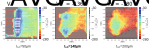
\includegraphics[width=\textwidth]{4_thinning/figures/cartosFautesNew.pdf}
    \caption{Fault susceptibility maps}
    \label{fig:fsm1}
\end{figure}
\begin{figure}[H]
    \centering
    \includegraphics[width=16cm]{4_thinning/figures/cartosFautesSpreading.png}
    \caption{Susceptibility area spreading}
    \label{fig:fsm1spread}
\end{figure}
\begin{figure}[H]
    \centering
    \includegraphics[width=16cm]{4_thinning/figures/cartosCouples.pdf}
    \caption{Fault susceptibility maps couples}
    \label{fig:fsm1couple}
\end{figure}
With geometric and electrical modeling complete, it is now possible to conduct actual experiments in order to verify the meaningfulness of the previous approaches.
In this context, three an STM32F439VIT6 LQFP100 identical targets were thinned to three different levels, from 750 µm to respectively 200 µm, 140 µm and 50 µm, respectively named ST200, ST140 and ST50 for the rest of this Chapter.
In order to verify the three conclusions extracted from the modeling section, three experiments are conducted for each target.

The first experiment aims at measuring the minimal voltage pulse amplitude $V_{PU}^{MIN}$ required to induce a faulty behavior on an IC performing computations.
These experiments are called Fault Susceptibility Maps (FSM).
They allow spotting the region where the IC is sensitive to BBI, no matter which type of induced fault.
Therefore, when mapping an entire IC, it is common to spot various areas not directly involved in the targeted calculation, like the analog voltage regulator or the FLASH memory logic control logic not to cite them all.
As a result, and because in a fault injection context the cryptographic core is very often targeted, it was decided to focus the maps above the STM32 AES core only.
Fig. \ref{fig:fsm1} presents the three performed FSM.
From left to right, $t_{SUB}$ goes from 50 µm, then to 140 µm, finally to 200 µm.
As stated before, the maps are performed above the hardware AES core of the IC, temporally aiming the penultimate AES round.
The scanned area measures 1.7 mm by 1.7 mm, with a displacement step of 40 µm between each point.
$V_{PU}$ was limited to the following range: [30 V ; 280 V], with 5 V steps and a negative polarity.
The pulse width was fixed at 6 ns.
The first important thing to note here is that, as predicted with the geometric and electrical modelings, a thinner substrate allows a lower fault induction threshold.
It is mainly shown thanks to the measurement of the average voltage required to induce a fault across the entire map, annotated at the top of each map.
All of this sustains the first conclusion made in section \ref{chap4:sect:geomModel}.

Then, the second experiment, whose results are shown in Fig. \ref{fig:fsm1spread}, consist in analyzing the spreading of the BBI susceptibility area.
The core of the experiment is identical as before.
However, in order to highlight the spreading effect, it was required to set a lower maximum voltage amplitude (in absolute value).
The value of 180 V was chosen as it is the average voltage of the medium-thinned IC.
What is interesting here is that, for the ST200 target, because the voltage at the epitaxy level cannot reach the threshold value $V_F$ in most cases, the fault area is tiny compared to the other targets, and focused on the AES core.
Then, concerning the ST140 target, thanks to the thinner substrate, the voltage at the epitaxy level can reach a higher value, and thus can cause more logic gates or further logic gates from the probe to have a faulty behavior.
Eventually, the ST50 target shows the largest fault area.
These experiments help to sustain the second conclusion of section \ref{chap4:sect:geomModel}.

Eventually, the last experiment consisted in finding, whenever possible, $(t_{SUB}, V_{PU})$ couples for which the susceptibility area is identical across all targets.
The search for the couples of values was done by first choosing an arbitrary couple for ST200 target, and then calculating the correlation for each couple between the other two susceptibility areas and finding the highest correlation.
Then, to confront the geometric modeling predictions, we calculated, thanks to equation \ref{chap4:sect:geomModel:eqnVpu*}, couples corresponding to